\section{FetchOrderables-Service}

\subsection{Allgemeines}

Damit der Nutzer alle angebotenen Menüs und Produkte in der App sehen und in weiterer Folge auch
bestellen kann, müssen diese bei App-Start per API-Requests geladen werden.\\
Hierfür gibt es nachfolgende Service-Funktionen.

\subsubsection{API-Routes}

\begin{code}
    \centering
    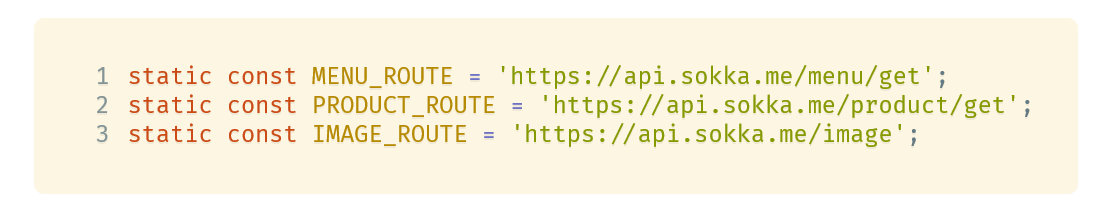
\includegraphics[width=1\textwidth]{images/Client/services/fetch-orderables/apiRoutes.png}
    \vspace{-25pt}
    \caption{Benötigte \lstinline{/menu}-, \lstinline{/product}-, und \lstinline{/image}-Routes der Sokka-API}
\end{code}

\subsection{Laden von verfügbaren Menüs}

Die API übermittelt alle Menüs per JSON-Format mit nur einem einzigen gesendeten Request, wodurch
durch eine einfache Iteration alle Menüs schnell in die App geladen werden können.

\begin{code}
    \centering
    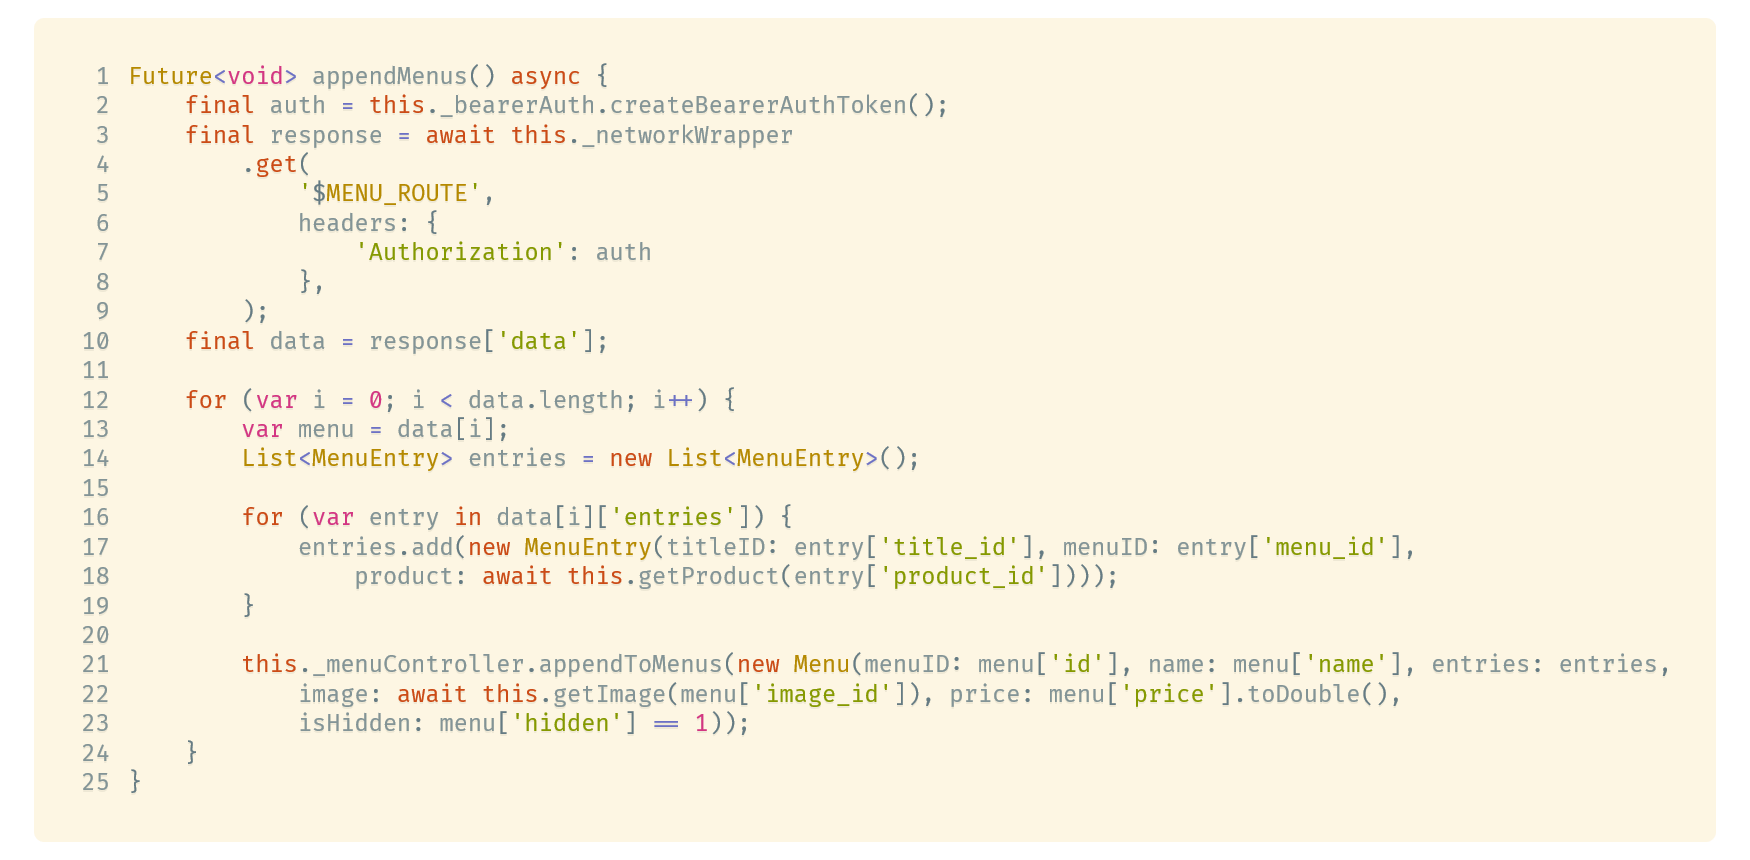
\includegraphics[width=1\textwidth]{images/Client/services/fetch-orderables/appendMenus.png}
    \vspace{-25pt}
    \caption{Abrufen und Speichern der verfübaren Menüs}
\end{code}

Aus den erhaltenen Response-Daten werden direkt neue Objekte vom \lstinline{Menu}-Model erzeugt,
dem Menu-Controller hinzugefügt und im Menu-View angezeigt.

\subsection{Laden von verfügbaren Produkten}

Das Abrufen der angebotenen Produkte erfolgt nach demselben Prinzip wie bei der Abfrage der Menüs.
Per API-Call werden alle Produkte übermittelt und können durch Iterieren über das JSON-Objekt
in die App geladen werden.

\begin{code}
    \centering
    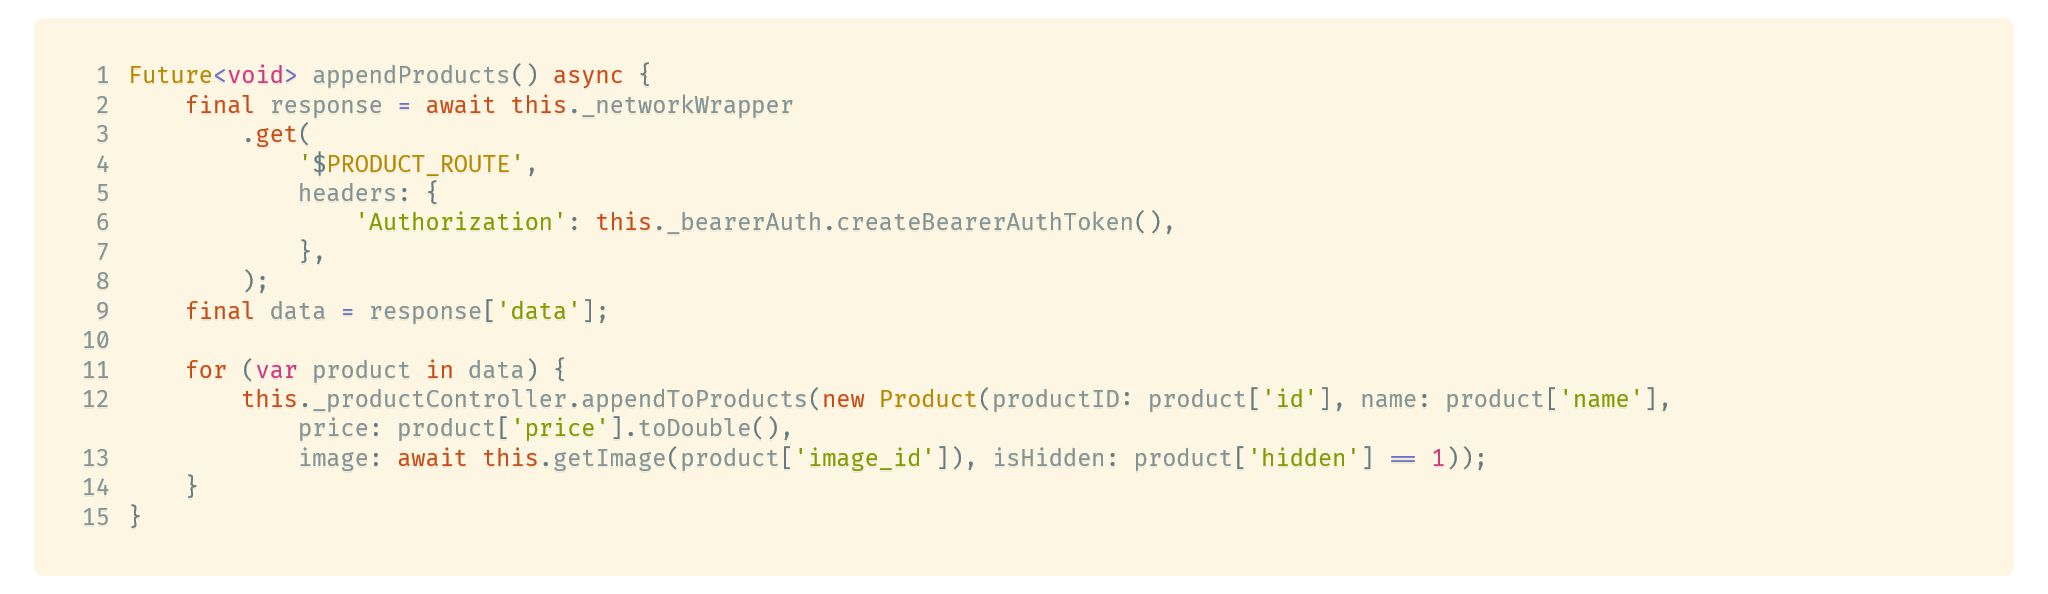
\includegraphics[width=1\textwidth]{images/Client/services/fetch-orderables/appendProducts.png}
    \vspace{-25pt}
    \caption{Abrufen und Speichern der verfügbaren Produkte}
\end{code}

\subsubsection{Wrapper-Funktionen für das Initialisieren der Menüs und Produkte}

Wie beim User-Authentication-Service gibt es auch für die Initialisierung aller Waren eine Wrapper-Funktion,
die bei Start der App aufgerufen wird.

\begin{code}
    \centering
    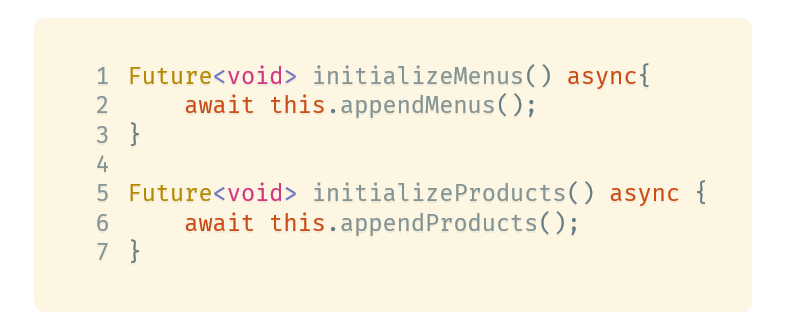
\includegraphics[width=1\textwidth]{images/Client/services/fetch-orderables/wrapperFunction.png}
    \vspace{-25pt}
    \caption{Abrufen und Speichern der verfübaren Menüs}
\end{code}

\newpage